\chapter{Designing the framework} \label{chapter:design}

Providing users with a high level of abstraction is not unheard of in the context of practical AI/ML platforms. Many software-as-a-service products offer features for hiding the technicalities of machine learning. However --- as we have discussed in Section \ref{section:existing} --- these tend to abstract away the details of both data science and AI engineering, overall hindering the development process. The design proposed here aims to tackle and simplify only the deployment-related concepts.

\section{Scope} \label{section:scope}

As highlighted by several case studies in Chapter \ref{chapter:background}, the transition from prototypes to production-ready systems is often named as the source of unexpected struggle. Maybe it is not a coincidence that a significant portion of the SE4ML best practices should be implemented in this phase. Unfortunately, it is easy to gloss over them while tackling the underestimated difficulties of this \textit{transition}. Therefore, the aim of \textit{GreatAI} is to ease this step of the lifecycle. Consequently, its scope is limited to the \textit{transition} step.

There have been attempts that at least partially address this issue; however, as we have seen in Chapter \ref{chapter:background}, these have limitations either from the perspective of best practices or stemming from their difficulty in being adopted. The scope has to be well-defined and limited to provide the best chance of providing an easy-to-adopt solution. To understand the API of a library, users first need to understand its aim and surface and have to become familiar with the problems it solves. Thus, focusing only on the \textit{transition} step seems reasonable. This step is highlighted in Figure \ref{fig:scope}.

\begin{figure}
    \centering
    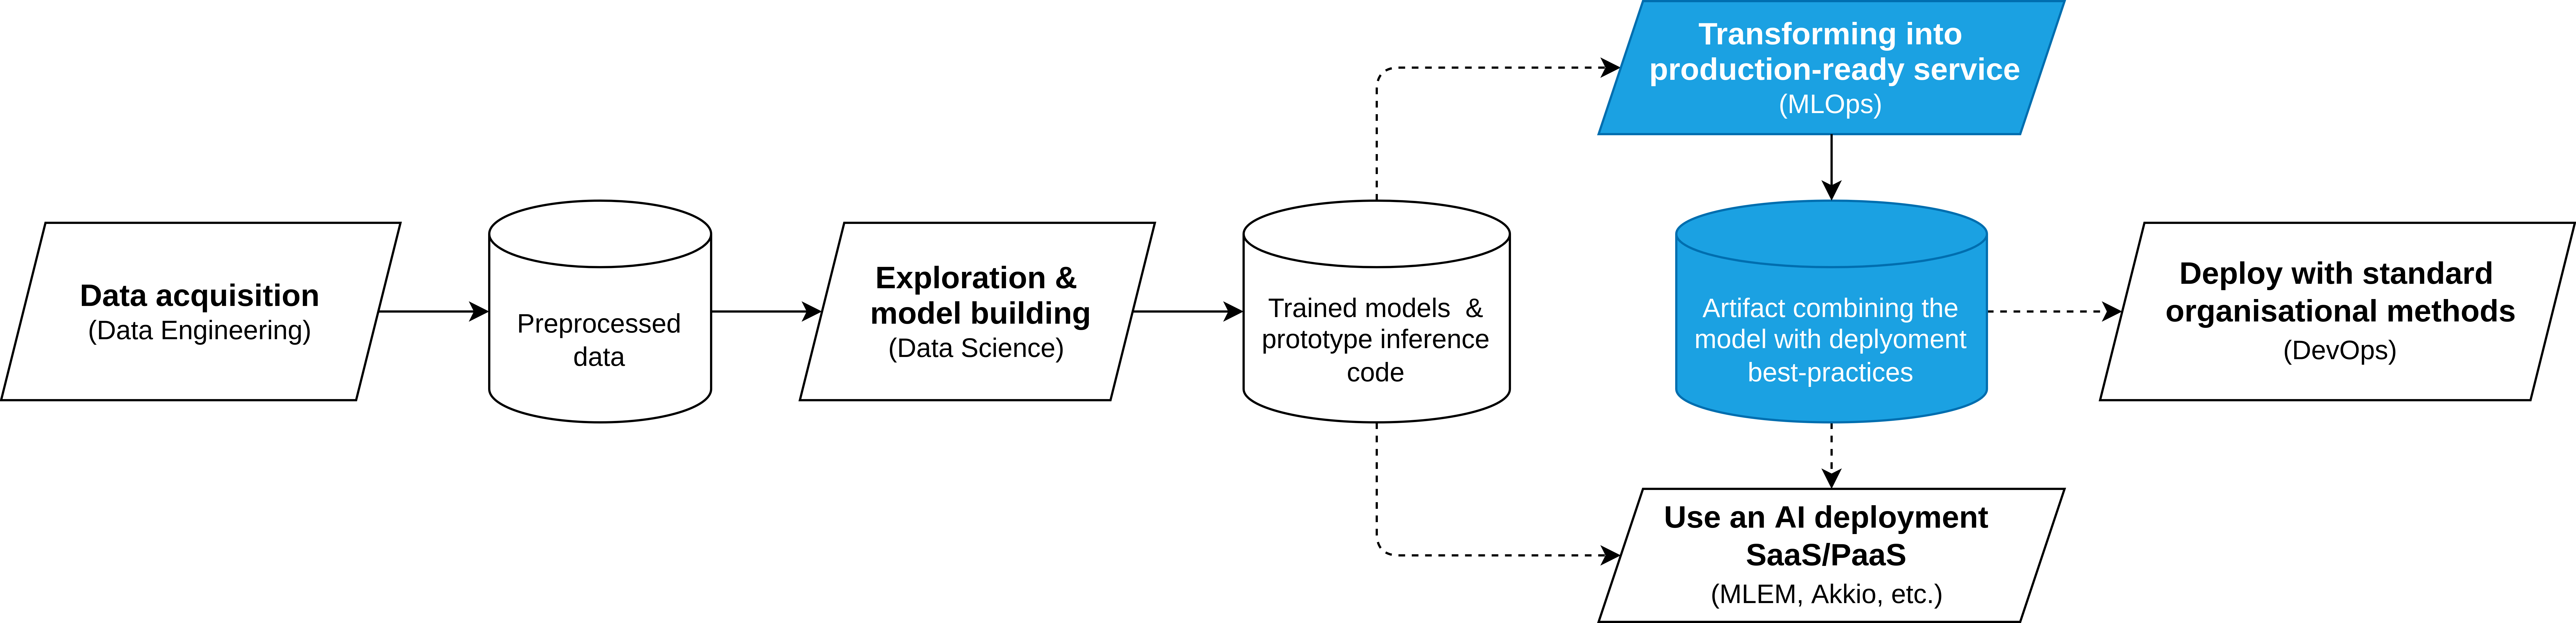
\includegraphics[width=\linewidth]{figures/scope.drawio.png}
    \captionsetup{width=.9\linewidth}
    \caption{Usual process steps (based on \cite{john2020architecting}) in the development lifecycle of a data-heavy software solution. The dashed arrows denote optional paths: after a prototype has been completed, there are multiple options for its deployment. The steps with blue background show the primary scope of \textit{GreatAI}.}
    \label{fig:scope}
\end{figure}

It is interesting to mention that \href{https://xkcd.com/927/}{there is a proliferation} of platform/software as a service (PaaS/SaaS) products for deploying AI\footnote{Such as \href{https://mlem.ai/}{MLEM}, \href{https://streamlit.io/cloud}{Streamlit} or any AutoML SaaS platform, for example, \href{https://www.akkio.com/role/software-engineers}{Akkio} as these often have a one-click deployment feature as well.}. At first, these may look intriguing. However, they tend to only focus on getting code easily deployed in the cloud: AI best practices are not prioritised in this setup. Nevertheless, in many cases, it may be a suitable option to use such a service, and these can also complement \textit{GreatAI} as illustrated in Figure \ref{fig:scope}: first, the prototype is transformed into a \textit{GREAT} service and materialised as a common software artifact implementing the best practices. Then, it is either deployed using a deployment SaaS or the organisation's existing software deployment setup.

\section{Requirements} \label{section:requirements}

The best practices (which are referenced throughout the thesis) with which the design is concerned are a subset of those compiled by Serban et al. \cite{serban2020adoption,serban2021practices} and John et al. \cite{john2020architecting}. The core requirements --- set of covered best practices --- for a software solution that has the potential to improve our problem context are presented in the following, along with some explanation and clarification for each of them.

\paragraph{General} Albeit not explicitly in the list of best practices, compatibility is vital in encouraging adoption. Large projects frequently end up depending on numerous packages, each of which may impose some restrictions on the code: since these all have to be satisfied simultaneously, this can result in severe constraints. 

The open-source scene of data-related libraries is vibrant. To take the example of data validation, there are at least four popular choices which offer varying but similar features: \href{https://github.com/SeldonIO/alibi-detect}{Alibi detect}, \href{https://github.com/PAIR-code/facets}{Facets}, \href{https://github.com/great-expectations/great_expectations}{Great Expectations}, and Data Linter \cite{hynes2017data}. The responsibility of choosing the most fitting solution falls on the user. Thus, they should not be limited in this by \textit{GreatAI}. 

The programming language (PL) of the library should be its only non-general property. Fortunately, the de facto PL for data science is Python, so implementing the library in it should not significantly limit its applicability.

\paragraph{Robustness} in software development can be achieved by preparing the application to handle errors gracefully, even unexpected ones \cite{bishop1998robust}. Errors can and will happen in practice: storing and investigating what has led to them is required to prevent future ones. In the case of ML, errors might not be as obvious to detect as in more traditional applications (see the above-mentioned data validators). Even if a single feature's value falls outside the expected distribution, unexpected results can happen. In cases where this might lead to real-world repercussions, extra care has to be taken to construct as many safeguards as practicable. \textit{GreatAI} should support its clients in this.

\paragraph{End-to-end} In this case, it refers to end-to-end feedback. That is, feedback should be gathered on the system's real-world performance, which should be taken into account when designing/training the next iteration of the model. Static datasets may fail to capture the changing nature of real life and can become outdated if they are not revised continuously. A well-packaged deployment should make it trivial to integrate new training data.

\paragraph{Automated} The available time of data scientists and software engineers is limited and expensive. For this reason, humans should only be involved when their involvement is necessary. Steps in the development process that can be automated without negative consequences must be automated in order to achieve efficient development processes and let the experts focus on the issues that require their attention the most.

\paragraph{Trustworthy} As detailed by the \href{https://digital-strategy.ec.europa.eu/en/library/ethics-guidelines-trustworthy-ai}{\textit{Ethics guidelines for trustworthy AI}}, human oversight, transparency, and accountability are some of the key requirements for trustworthy AI applications. For increasing public acceptance and trust while minimising negative societal impact, trustworthiness is essential.

The requirements were chosen stemming from their general importance and potential to be mostly handled (implemented) by a software framework. That is why these provide an ideal initial direction for tackling the issue. Of course, these do not cover all best practices; for instance, the ones relating to organisational processes fall outside the realm of computer science.

\section{Design principles} \label{section:principles}

Before diving into the concrete issues solved, let us detail the principles that should be used for implementing them in the scope of this framework. As implied in Section \ref{section:scope}, the Unix philosophy \cite{ritchie1978unix,salus1994quarter} of software design is followed. Most notably, the design goal that encourages to \textit{write programs that do one thing and do it well.}\footnote{\textit{Write programs to work together} is also applicable since allowing interoperability is part of the core requirements.}. Apart from providing a clear and simple picture of the intended use cases for the library, this is also in line with the main notion of \textit{A Philosophy of Software Design} \cite{ousterhout2018philosophy}: APIs should be narrow and deep. A narrow width refers to having a small exposed surface area, i.e. having a small number of functions and classes in the public API. In contrast, depth implies that each accomplishes an involved, complex goal. 

In a way, the width of an API is the price users have to pay (the effort required for learning it) to use it, while the depth is analogous to the return they get from it. Having to learn little and being provided with a lot of functionality maximises return on investment (ROI), hence, developer experience (DX). The theoretical frameworks presented in \textit{The Programmer's Brain} \cite{hermans2021programmer} provides us with explanations and vocabulary from psychology for arguing about the cognitive aspects of API design. In the following, two of them will be used for detailing the design principles: cognitive dimensions of code bases (CDCB) which is an extension of the cognitive dimensions of notation (CDN) framework \cite{blackwell2001cognitive}, and linguistic anti-patterns \cite{arnaoudova2016linguistic}. The former comes with a set of dimensions describing different (often competing) cognitive aspects of code that influence one's ability to perform specific tasks.

Linguistic anti-patterns provide guidelines for improving consistency and decreasing the false sense of consistency when there is none. Also, choosing the right names for identifiers can help activate information stored in the long-term memory, making it quicker to comprehend and easier to reason about the code \cite{deissenboeck2006concise}. Finding the most accurate and useful names is more challenging than it first seems. Accuracy and usefulness are already often competing goals. The more precise the name, the longer and therefore less convenient to use \cite{butler2009relating}. In short, good names are essential to good APIs; consciously considering the implications of names should be an integral part of the design process.

Nonetheless, simple APIs come at a high technical cost. The library has to implement these in a way that still allows for high performance in production \cite{kleppmann2017designing} and avoids being tied to specific libraries or technologies. Inspiration for the latter may be gained from the ML pipelines of Prado et al. \cite{prado2020bonseyes}: they show that more freedom can be achieved with plug-and-play steps and preconfigured defaults. 

\subsection{Default configuration}

Existing frameworks frequently suffer from the entanglement of numerous levels of abstractions.\footnote{\href{https://grugbrain.dev/\#grug-on-apis}{grugbrain.dev}} Instead of exposing each implementation detail and encouraging users to interact with most of them, many of these could be abstracted away in a more high-level layer. Even where configuration may be helpful for advanced users, default values can still be chosen automatically while providing an override option where necessary.

For example, tracing the evaluations and the model versions used in a distributed fashion is very much expected of a trustworthy system. Hence, turning this feature on by default but allowing opting-out from it can result in less scaffolding required from the library's users. It also decreases their up-front cognitive load, which by definition flattens the learning-curve \cite{hermans2021programmer}. Similar features can be imagined for providing a service API for the algorithms, giving feedback, marking outliers, and more.

Being \textit{automated} is listed as a requirement, but it is imperative to only automate for simplifying and not for hiding decisions. More precisely, guessing must not be a part of automation. For instance --- an otherwise handy WebGL library --- TWGL.js, has a feature for automatically guessing the type of vectors based on their names. Suppose it matches the \texttt{/colou?r/i} pattern. In that case, it is treated as a vector with three components\footnote{\href{https://github.com/greggman/twgl.js/blob/e3a8d0ed09f7f5cd4be0e4cb5976081c2b5013aa/src/attributes.js\#L139}{\tiny github.com/greggman/twgl.js/blob/e3a8d0ed09f7f5cd4be0e4cb5976081c2b5013aa/src/attributes.js\#L139}}. It is easy to imagine that this can help in certain scenarios. Still, it does so at the cost of immense confusion when correctly renaming a variable breaks the application. In CDCB, this equates to scoring high on the dimension of \textit{Hidden dependencies} and low on \textit{Visibility}.

Learning from this, any guessing must be avoided to create a pleasant API. However, this conflicts with providing defaults for each configuration value. Even if these would be reasonable defaults derived from educated guesses, they are still merely guesses. Nevertheless, if the users were required to specify each configuration option, that would lead to vastly more boilerplate code. This verbosity is captured by the \textit{Diffuseness} dimension of CDCB and, of course, should be minimised.

To resolve this conflict, \textit{GreatAI} should have recommended values instead of defaults. This can mean a context object (as suggested in \cite{ousterhout2018philosophy}), which contains the result of each design consideration that has to be made for a service's deployment. If not configured manually, the recommended values are applied automatically, just like defaults. The values chosen for each parameter must be clearly highlighted. Coming from the library's single responsibility, the number of parameters should not be immense; hence, the user can be expected to comprehend them instead of just being overwhelmed and skipping them.

This way, the library attempts to notify its user about the existence of these decisions but does not force them to decide manually. As a result, no initial configuration is needed for starting out with the library (high \textit{Provisionality}, low \textit{Diffuseness}), and the dependencies are not hidden since they are explicitly highlighted.

\subsection{Documentation}

Little value can be derived from software without good documentation; undoubtedly, good documentation is a prerequisite for adoption. Documentations come in many shapes: modern integrated development environments (IDEs) tend to show a popup of a function's description when requested (for instance, on mouse hover), and at the same time, a more comprehensive online manual and example projects are also still expected. Descriptive error messages can also be viewed as documentation.

The library must have quality documentation for all categories. Accordingly, for structuring it, the \textit{Diátaxis} philosophy is preferred \cite{Procida_Diataxis_documentation_framework} which prescribes dividing documentation into 4 parts along 2 axes: practical-theoretical and passive-active consumption. The four quadrants derived from this are tutorials, how-to guides, references, and explanations.

Once again, we might notice two competing interests: the level of detail and the length of the documentation. For example, FastAPI\footnote{\href{https://fastapi.tiangolo.com/async/\#concurrent-burgers}{fastapi.tiangolo.com}}, a popular Python web framework, has extensive descriptions and explanations on all topics related to Python's import system, the HTTP protocol, concurrency, deployment, and more. The actual framework's documentation is sprinkled over these overly broad topics. This is undoubtedly helpful for beginners to acquire knowledge from a single place. Yet, this high level of accessibility actually hinders the process of finding the relevant sections; in CDCB, this shows a trade-off between the support of \textit{Searching} and \textit{Comprehension} tasks. Diátaxis' take is that linking to external resources about the library's domain is welcome, but the documentation must have a single responsibility: describing the library itself.

A large portion of software documentations is automatically generated from source code, and this has the advantage of always keeping it in sync with code changes. However, it might also signal that the API is too large because it is inconvenient for the developers to document it by hand. Striking the right balance between handcrafted and automatically extracted documentation may be a vital component of good documentation.

When it comes to example code, showing at least a minimal starter code and the way of customising it has to be showcased front and centre. It is a well-known observation that developers only read the documentation when they are stuck, and there might be some merit to this. Making them not get stuck --- by providing a starter code from which they can explore the API using IntelliSense-like solutions --- should be preferred. Take the example of another widely popular Python web framework, Flask\footnote{\href{https://flask.palletsprojects.com/en/2.1.x/}{flask.palletsprojects.com/en/2.1.x}}, at this time, has 324 homogeneously styled links on its landing page. Out of these, only two lead to the quick-start code. Of course, it is not hidden, but I argue that the DX could be improved by displaying where to start more prominently.

\subsection{Developer experience}

Subjectively, a key component of good DX is \textit{Progressive evaluation} through which development can become a highly iterative, experimental process. This is well-understood by popular data science tools, such as Jupyter Notebooks. \textit{GreatAI} also has to support some level of this, for example, in the form of auto-reload on code changes. Further key ingredients for good DX are consistency and discoverability. To give one more example, the MySQL connector's Python implementation\footnote{\href{https://dev.mysql.com/doc/connector-python/en/}{dev.mysql.com/doc/connector-python/en}} has a cursor object which exposes a \texttt{fetchone} method. Even though this naming scheme is not conventional in Python since it does not follow \href{https://peps.python.org/pep-0008/}{PEP 8}, at least the API is intuitive: changing \texttt{sql\_cursor.fetchone()} to \texttt{sql\_cursor.fetchall()} returns all items instead of just one. Using good and consistent names is the key to good DX.

At the same time, Python codebases are rarely strictly object-oriented (OO). They are a mix of the functional, data-driven, and OO paradigms. Consequently, relying on classes for grouping related functions is not always desirable; therefore, it is even more imperative to name similar functions similarly. This helps discoverability and chunking \cite{hermans2021programmer}, which amounts to quicker comprehension.

There is one more reason to prefer consistency: humans have limited short-term memory (STM) \cite{miller1956magical}. Even though flags as function parameters are frowned upon by some \cite{martin2009clean}, they are useful, especially when configuring libraries. However, if there is no convention for the default value of a flag, clients have to remember the flag's name and initial value simultaneously, quickly overloading their STM. Thus, in the codebase, all defaults must be the same, let us say, \texttt{False}. Sometimes, it can result in a \textit{disable} prefix, which may turn into a double negation. Nevertheless, users should never encounter this since the doubly-negated version is the default; thus, it is only singly negated when overriding it. This approach also implies that something may be recommended to be turned on by default.

\section{Architecture} \label{section:architecture}

Although API design has been the central subject so far, it is worth remembering that APIs are usually expected to have corresponding implementations. \textit{GreatAI} is no exception. As laid out in Section \ref{section:principles}, we strive for narrow and deep interfaces; thus, it is time to address the \textit{depth} component.

\textit{GreatAI} stands on the shoulders of numerous open-source packages and integrates them to provide its various features. The most fundamental dependencies and the entire library in context are shown in Figure \ref{fig:technologies}. Given a Python script or a Jupyter notebook, \textit{GreatAI} transforms the specified prediction functions into a production-ready deployment, deployable either as a Docker image, WSGI-server, or an executable relying on \texttt{uvicorn}. The complete list of dependencies can be found in the repository\footnote{\href{https://github.com/schmelczer/great-ai/blob/main/pyproject.toml}{github.com/schmelczer/great-ai/blob/main/pyproject.toml}}.

\begin{figure}
    \centering
    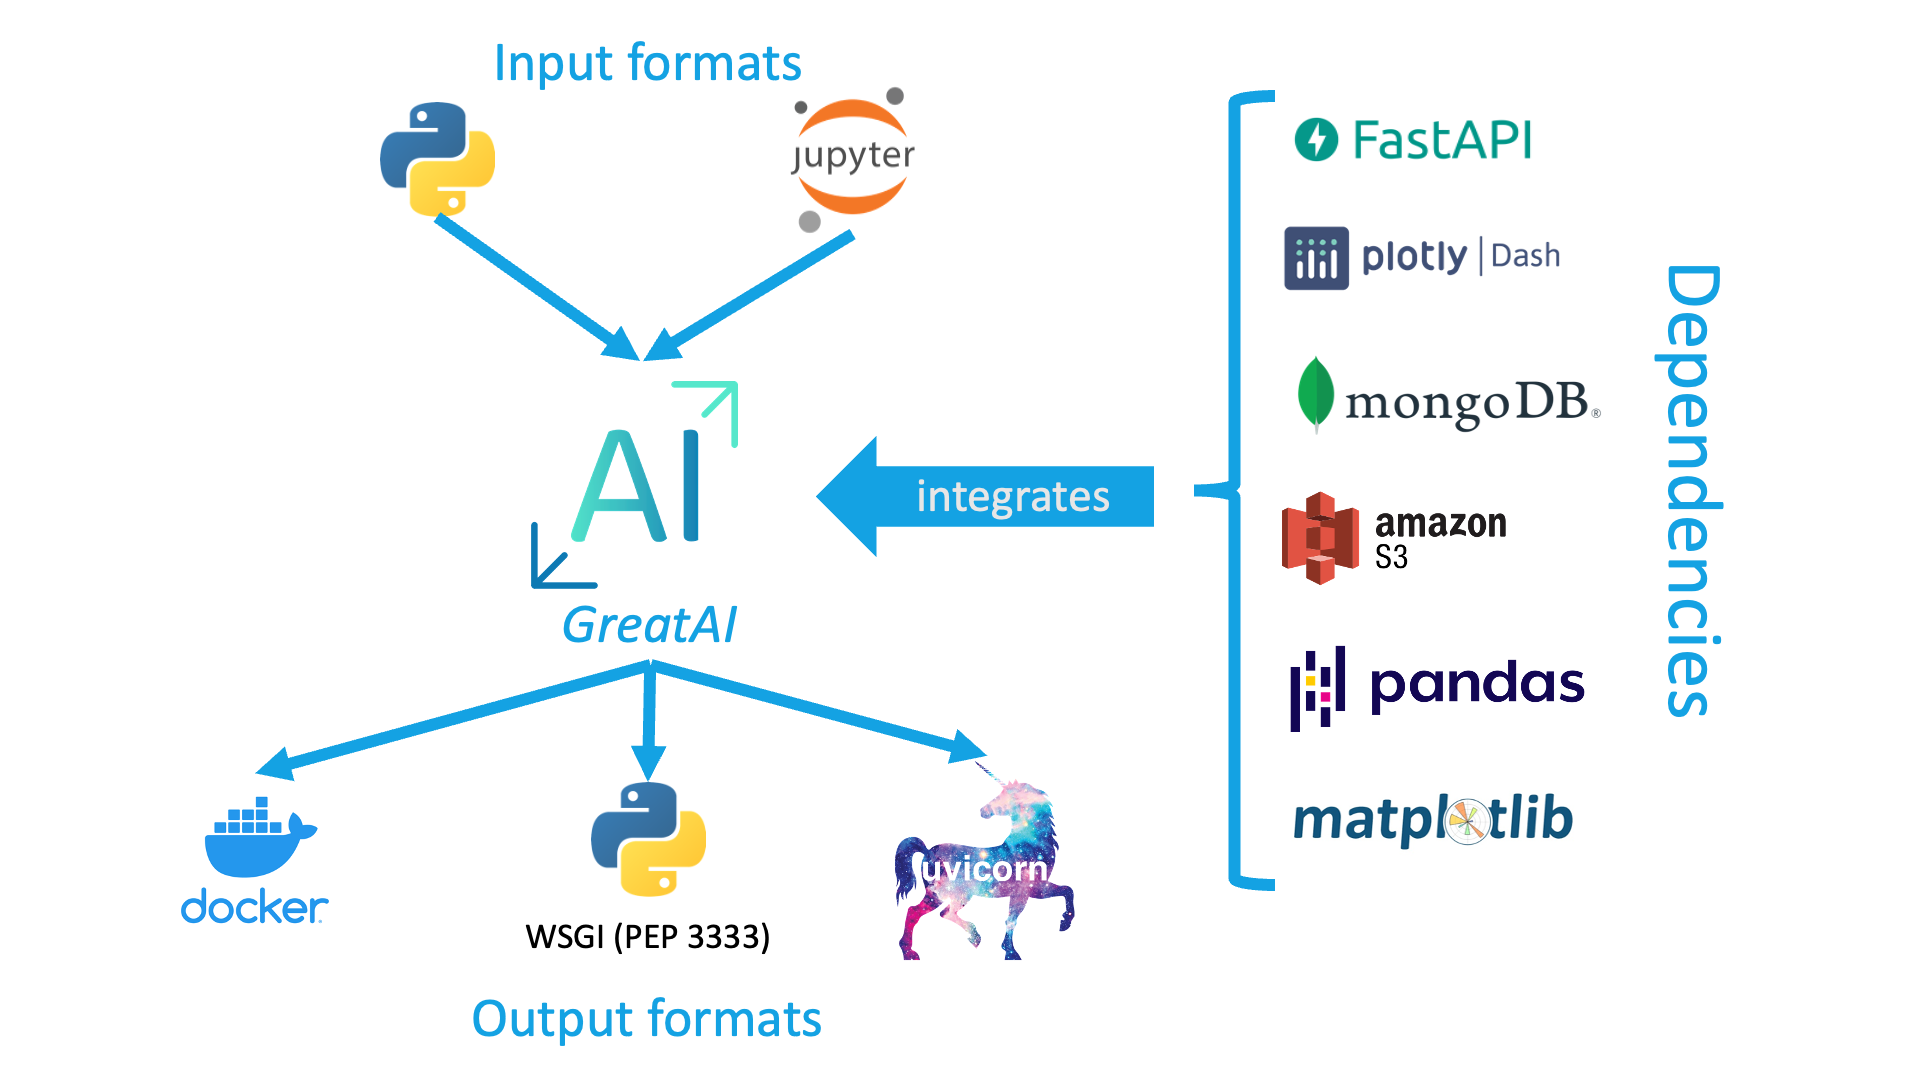
\includegraphics[width=0.65\linewidth]{figures/technologies.png}
    \captionsetup{width=.9\linewidth}
    \caption{A very high-level overview of \texttt{GreatAI} in its context. The main dependencies are also highlighted.}
    \label{fig:technologies}
\end{figure}

The general theme in the implementation is that each explicit best practice should have its distinct, loosely-coupled functions or classes. When collaboration opportunities arise, such as persisting the model versions (\nth{1} component) into prediction traces (\nth{2} component), there are three primary conduits for realising them. These are the \texttt{context} object responsible for the global configuration per process, the \texttt{FunctionMetadataStore} specifying the expected behaviour of each prediction function, and finally the \texttt{TracingContext} that is created anew for each prediction input (session).

After refining the framework with feedback gathered from case studies and users, we will end up with the core architecture presented in Figure \ref{fig:architecture}. The implementation is mixed-paradigm, combining the expressiveness of functional and the design patterns of object-oriented programming (OOP) in order to maintain an overall low complexity. Reflection is also utilised, especially for run-time type-checking and generating the API definitions and Dashboard components. Regardless, the architecture is still presented with a syntax similar to the class diagrams of UML2 \cite{Rumbaugh2004} because it provides the freedom to express even the non-OOP design aspects.

For the sake of brevity, Figure \ref{fig:architecture} does not show all fields, and some related entities have been combined, e.g. the \textit{GroundTruthAPI} box represents the \texttt{add\_ground\_truth}, \texttt{query\_ground\_truth}, and \texttt{delete\_ground\_truth} functions. The client project can also access most of the presented entities, but these optional dependency arrows are not shown in the diagram. The \texttt{utilities} submodule is also left unexpanded; almost all of its functions are orthogonal with the exception of \texttt{parallel\_map}. The latter follows a textbook producer-consumer model facilitated by queues and event signals \cite{wang2020producer}.

\begin{figure}
    \centering
    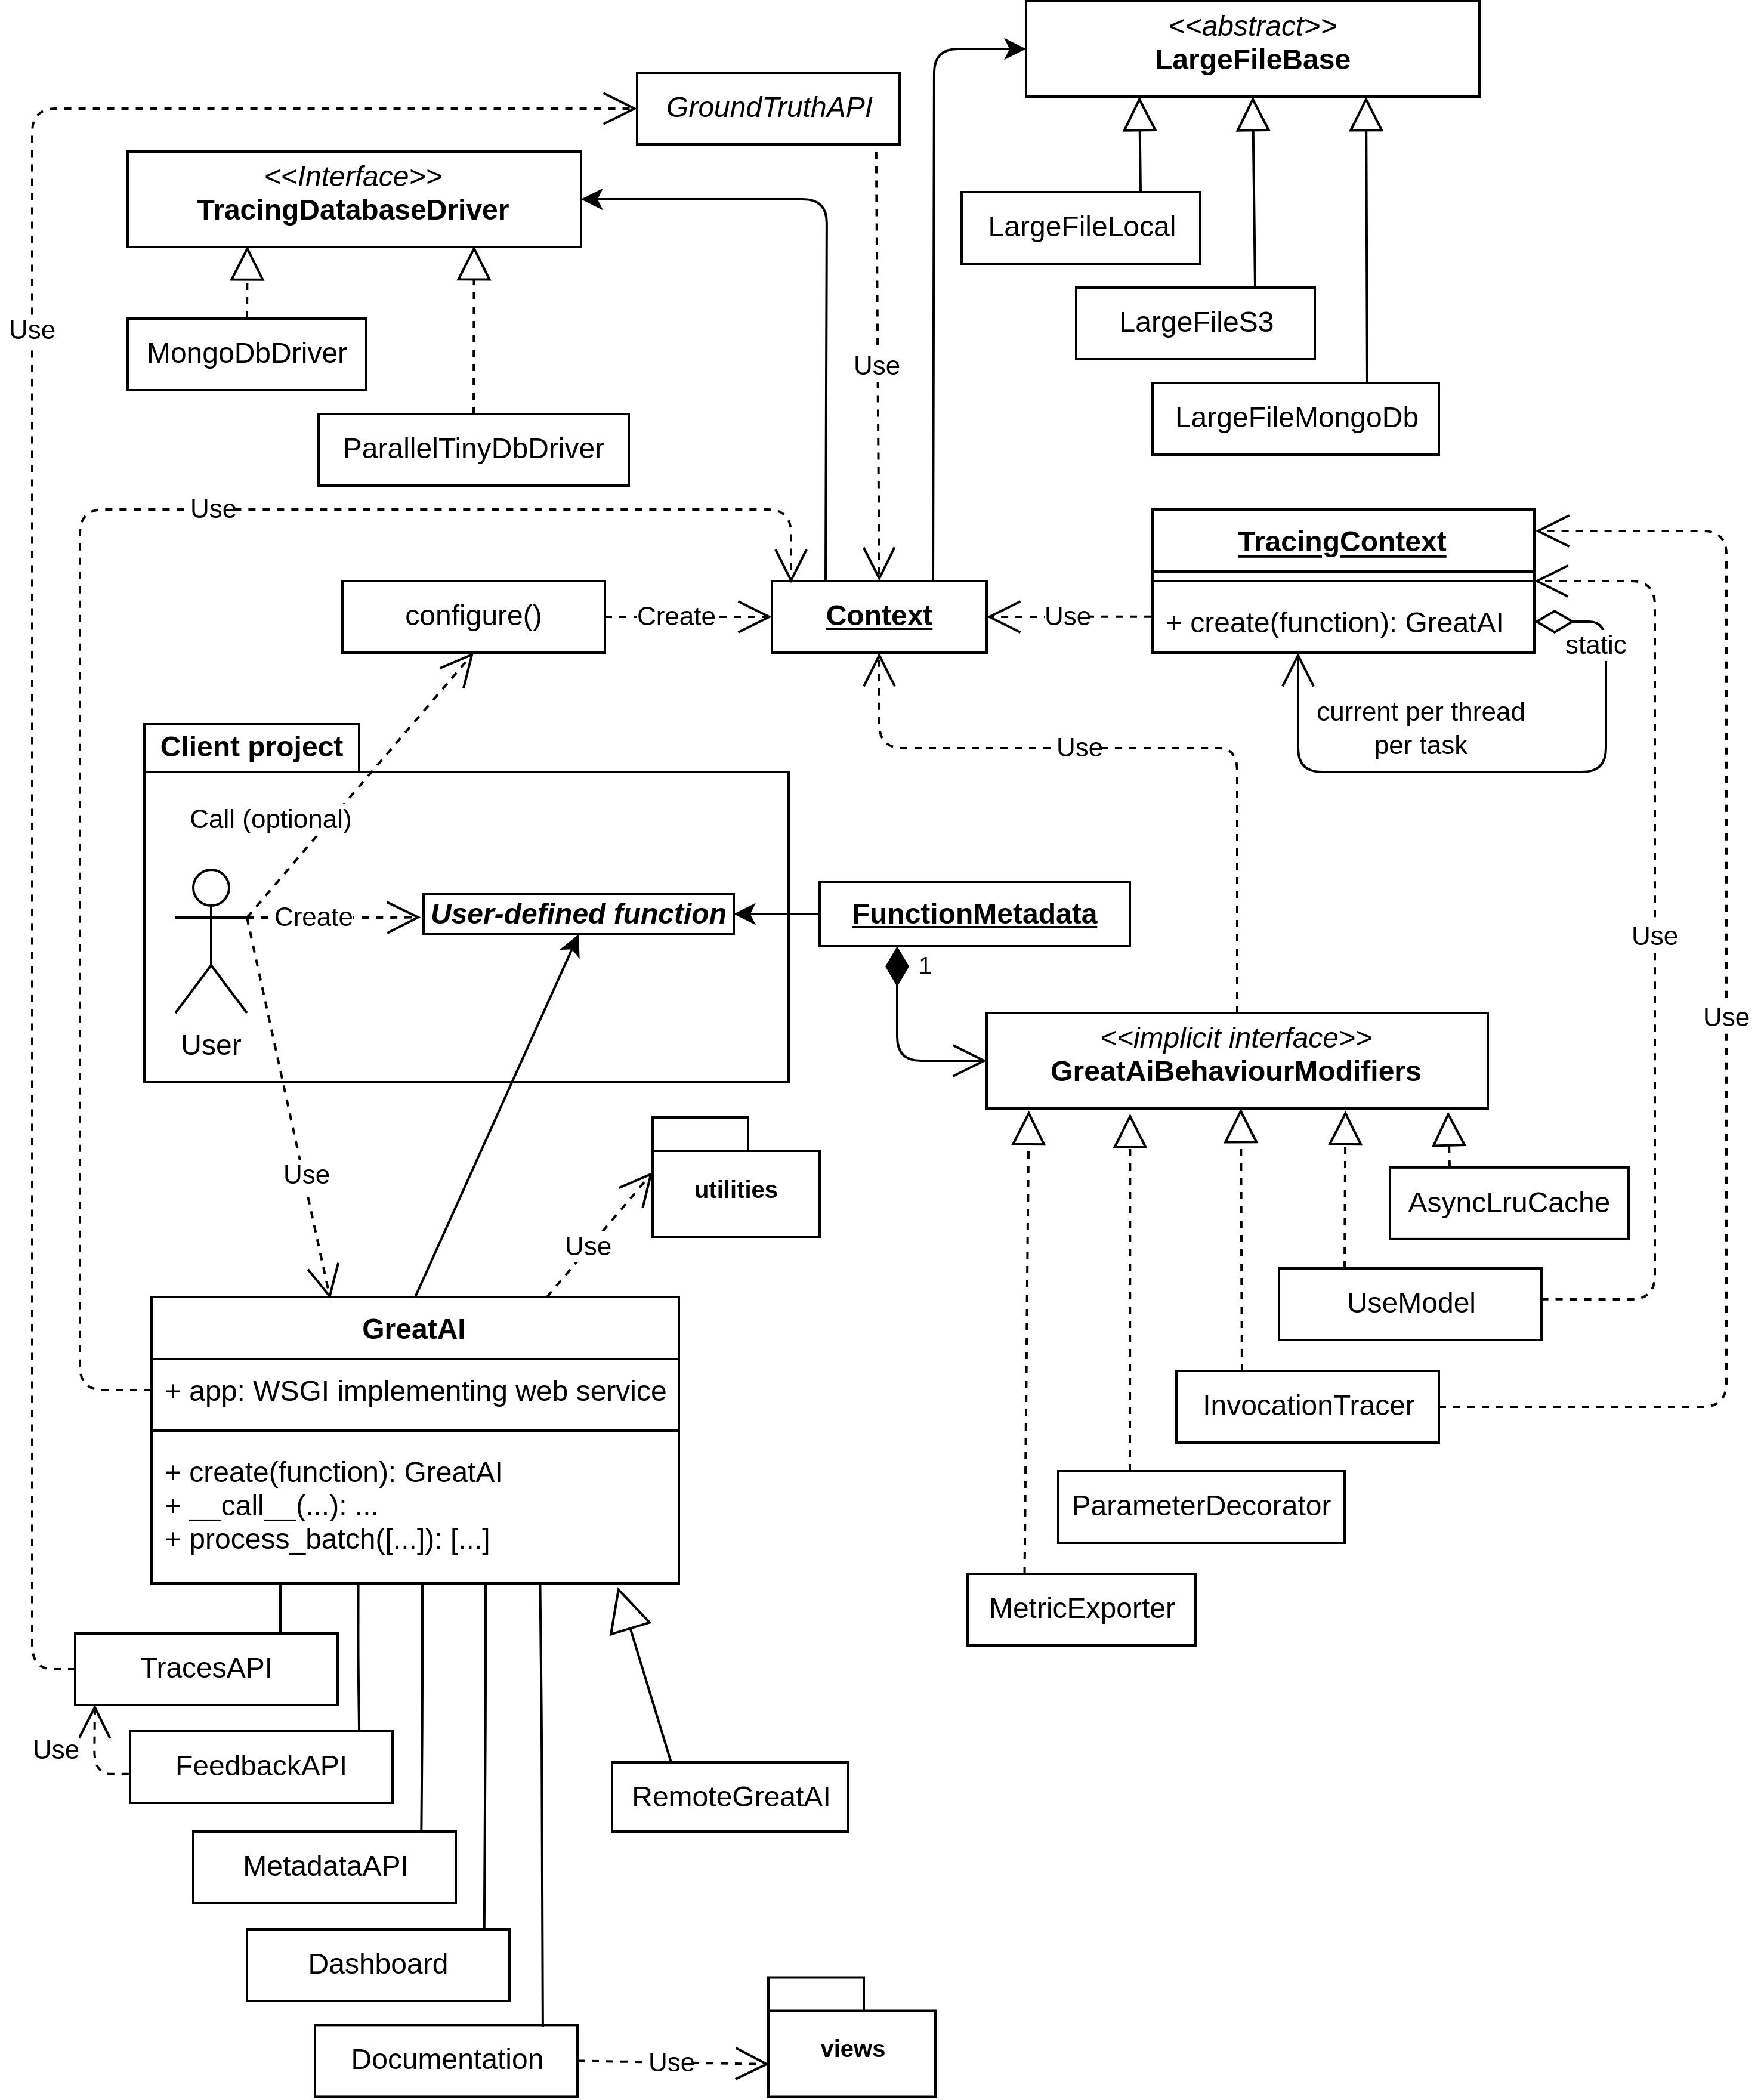
\includegraphics[width=\linewidth]{figures/architecture.png}
    \captionsetup{width=.9\linewidth}
    \caption{The core architecture of \textit{GreatAI} illustrated with syntax loosely-based on UML2 \cite{Rumbaugh2004}. Given its framework nature, the expected client project and the actor integrating it are highlighted; the associations between the framework and the client project are achieved through the use of decorators.}
    \label{fig:architecture}
\end{figure}
